\chapter{色谱}

\begin{introduction}
	\item 基本概念与术语(理解)
	\item 塔板理论和速率理论(掌握)
	\item 气相色谱仪的结构、检测器特点、检测方法(掌握)
	\item 高效液相色谱法的特点(了解)、主要部件及分析流程(熟悉)
	\item 几种色谱法的应用特点(熟悉)
	\item 色谱技术在生物分析中的应用(了解)
\end{introduction}


%设计方案:
%1.定义、概念、原理,做个环境
%2.公式、符号说明环境
%3.步骤、结构、小点:列表
%4.对比:表格



\section{色谱基本概念与术语}
%1、理解基本概念与术语:
%色谱流出曲线 (chromatogram):指样品注入色谱柱后,信号随时间变化的曲线。

\subsection{分类}
色谱(Chromatography) 法是一种重要的分离分析方法,它是根据组分在两相中作用能力不同而达到分离目的的。
\begin{itemize}
	\item 按流动相分:气相色谱(GC)、液相色谱(LC)、超临界流体色谱(SFC);
	\item 按机理分:吸附色谱、分配色谱、离子交换色谱、排阻色谱等等;
	\item 按固定相在支持体中的形状分:柱色谱、平板色谱(纸色谱 薄层色谱);
	\item 按按分离效率分:经典液相色谱和高效液相色谱(HPLC)。
\end{itemize}

研究核心:选择最合适的色谱体系和条件,在最短的时间内达到最佳的分离效果。

\subsection{概念}

\begin{enumerate}
	\item 色谱流出曲线 (chromatogram):指样品注入色谱柱后,信号随时间变化的曲线(一般为高斯分布曲线)。
	\item 基线:无组分通过色谱柱时,检测器的噪声随时间变化的曲线。
	\item 峰宽:峰底宽$W_b$、峰半宽$W_{1/2}$、标准偏差$\sigma$的关系是(如图\ref{fig:chp1peak})
	\begin{gather*}
		W_b=4\sigma\\
		W_{1/2}=2\sqrt{2\ln 2}\sigma
	\end{gather*}
	\begin{figure}[!h]
		\centering
		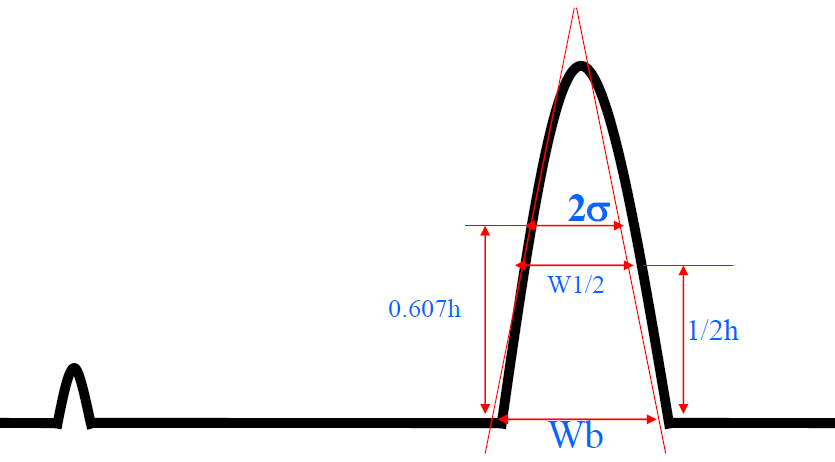
\includegraphics[width=0.45\linewidth]{image/chp1_peak}
		\caption{色谱峰示意图}
		\label{fig:chp1peak}
	\end{figure}
	\item 保留值
	\begin{itemize}
		\item 保留时间\footnote{保留:retention}$t_R$:进样到出现色谱峰的时间。
		\item 保留体积$V_R$:进样到出现色谱峰时消耗的流动相体积。
		\item 死时间$t_0$($t_M$):流动相流过色谱柱的时间。(另一种理解是不被固定相吸附的组分如甲烷、空气的保留时间。)
		\item 死体积$V_0$($V_M$):色谱柱的空隙体积。
		\item 校正保留时间:$t’_R=t_R+ t_0$。
		\item 校正保留体积:$V’_R=V_R- V_0=t_R\times F$,$F$是流动相线速度。
	\end{itemize}
		
	校正:死时间/死体积反映柱和仪器系统的几何特性,与被测组分性质无关,故通过校正来更好地反应被测组分的保留特性。
	\item 相对保留值
	
	某一组分1的校对保留值和标准物2的校对保留值之比,称为组分1对2的相对保留值。相对保留值仅随柱温及固定相变化。
	\begin{equation*}
	r_{1,2}=\dfrac{t'_{R_1}}{t'_{R_2}}=\dfrac{V'_{R_1}}{V'_{R_2}}
	\end{equation*}
	\item 分配系数与分配比(容量因子)
	分配系数$K$:一定$T$、$p$,两相达平衡后,组分在固定相和流动相\footnote{流动相:moving phase;固定相:stationary phase}浓度的比值。	
	\begin{equation*}
		K=\dfrac{C_s}{C_m}
	\end{equation*}
	
		分配比$k$:一定$T$、$p$,两相达平衡后,组分在固定相质量($p$)和流动相质量($q$)的比值。
	\begin{equation*}
	k=\dfrac{p}{q}
	\end{equation*}
	
	$K$与$k$的关系\footnote{注意:是同一组分,所以才有$c=p/V$}:
	\begin{equation*}
	K=\dfrac{C_s}{C_m} =\dfrac{p⁄ V_s}{q⁄ V_0}=k \dfrac{V_0}{V_s}
	\end{equation*}
	$k$与保留值的关系:
	\begin{gather*}
		k=\dfrac{t'_R}{t_0} =\dfrac{t_R-t_0}{t_0}\\
		t_R=t_0 (1+k)		
	\end{gather*}
	
	\item 分离效能的指标
	\begin{itemize}
		\item 选择性(相对保留值):相对保留值越大,选择性越好。仅由两组分热力学性质决定,与色谱柱无关。
		\item 峰宽度
		\item 分离度:考虑了保留时间和峰宽度,是一个综合指标。
		\begin{theorem*}{分离度}{}
			\begin{equation*}
			R=\dfrac{t_{R_2}-t_{R_1}}{(W_{b_2}+W_{b_1})/2}
			\end{equation*}
		\end{theorem*}
		
				
		\begin{itemize}
			\item $R<1.0$,两峰明显重叠;
			\item $R=1.0$,两峰达97.7\%分离;
			\item $R\geqslant 1.5$,两峰完全分开。
		\end{itemize}
	\end{itemize}
\end{enumerate}

\section{色谱两大理论}
%2.色谱两大理论—塔板理论和速率理论。塔板理论描述色谱流出曲线的方程,并通过这一方程各参数来研究影响分离的因素,要会计算。速率理论(van Deemter方程)是描述提高柱效的途径,理解范第姆特方程中各参数的含义?

\subsection{塔板理论}
\begin{itemize}
	\item 目的:从理论上得出描述色谱流出曲线的方程,并通过这一方程各参数来研究影响分离的因素。
	\item 两大假设:色谱柱存在多级“塔板”,每级塔板包含一个流动相和固定相,各自含一定量的各种组分;每种组分通过时,\textbf{在每级塔板处,两相间达到一次平衡}。
\end{itemize}

设某一组分的分配比$k=\frac{p}{q}$,经过一次转移(流到下一个塔板)后,0级塔板上组分的百分含量为$p'=\frac{p}{q+p}=\frac{k}{1+k}$,1级塔板上组分的百分含量为$q'=\frac{q}{q+p}=\frac{1}{1+k}$。经多次转移,组分在各级塔板的百分含量将符合二项分布,即${(p'+q')^N}$,$N$为转移次数。任一级塔板$r$对应的百分含量为:

\begin{equation*}
	f_{N,r}=\dfrac{N!}{r!(N-r)!} {(\dfrac{1}{1+k})}^r {(\dfrac{k}{1+k})}^{N-r}
\end{equation*}
以此作图即得流出曲线。

$N$特别大时,将呈正态分布:
\begin{equation*}
	C=C_{max}\times \mathrm{exp}\{-\dfrac{n(t_R-t)^2}{2t_R^2}\}
\end{equation*}

$C_{max}$其实就是峰高。对比标准正态分布曲线得:
\begin{equation*}
	{\sigma}^2=\dfrac{t_R^2}{n}
\end{equation*}

由$W_b$,$W_{1/2}$与$\sigma$的关系,得理论塔板数$n$的计算方法:

\begin{theorem*}{塔板数计算公式}{}
	\begin{equation*}
	n={\left(\dfrac{t_R}{\sigma}\right)}^2=16{\left(\dfrac{t_R}{W_b}\right)}^2=5.54{\left(\dfrac{t_R}{W_{1/2}}\right)}^2
	\end{equation*}
	注意$t_R$是热力学常数。
	
	有效塔板数$n_{eff}$为:
	\begin{equation*}
	n_{eff}={\left(\dfrac{t'_R}{\sigma}\right)}^2=16{\left(\dfrac{t'_R}{W_b}\right)}^2=5.54{\left(\dfrac{t'_R}{W_{1/2}}\right)}^2
	\end{equation*}
	
	$n$与$n_{eff}$的关系为:$$\dfrac{n_{eff}}{n}={\left(\dfrac{k}{k+1}\right)}^2$$
\end{theorem*}

小结:影响色谱柱效率的是理论塔板数$n$,$n$越大,色谱峰越窄,分离效率越好。色谱分离不限于液-固相,也可是气-液相。从理论上可以通过该方程预测具有不同分配系数$K$的两种物质在塔板数为$n$的色谱柱上分离的情况。

备考时,需要大家理解两个理论中公式的含义,并掌握计算的方法。
\begin{example}
	sf
\end{example}


\subsection{速率理论}
塔板理论的缺陷:半经验性理论;忽略了纵向扩散的影响;假设不可能完全实现;无法给出影响塔板高度的因素等。

\begin{theorem*}{Van Deemter方程}{}
	\begin{equation*}
		H=A+\dfrac{B}{u}+Cu
	\end{equation*}
	$u$是流动相线速度。$H$为塔板高度,$H=L/n$,$L$为色谱柱长。$H$越小,$n$越大,分离效率越好。
\end{theorem*}

\begin{enumerate}
	\item $A$是涡流扩散项:固定相填充不均匀引起的峰展宽,与颗粒直径正相关。使用较细粒度和颗粒均匀的填料,并尽量填充均匀,可减少涡流扩散,提高柱效。对于空心毛细管柱,$A$项为$0$。
	\begin{equation*}
		A=2\lambda d_p
	\end{equation*}
	$\lambda$:填充的不规则因子;$d_p$:固定相颗粒粒径
	\item $\frac{B}{u}$是纵向分子扩散项:由浓度差引起,分子延纵向扩散形成的展宽。由于组分在液相中扩散系数很低,因此液相色谱中可忽略$B$。
	\begin{equation*}
		B=2rD_m
	\end{equation*}
	$r$:弯曲因子(填充柱$r<1$,空心柱$r=1$),$D_m$:组分在流动相的扩散系数
	\item $Cu$是传质阻力\footnote{传质:溶解、扩散、转移的过程。传质阻力:影响传质过程的阻力。}项:组分在流动相和固定相之间传质的阻力。在非平衡状态下使有些分子较快向前移动,而另一些滞后,引起峰展宽。
	\begin{equation*}
		C=q\dfrac{k}{(1+k)^2}\dfrac{d_f^2}{D_s}+\omega\dfrac{k}{(1+k)^2}\dfrac{d_p^2}{D_m}
	\end{equation*}
	两项分别为固定相和流动相传质阻力。
\end{enumerate}

$H$对$u$求导可推出:
\begin{gather*}
	H_{min}=A+2\sqrt{BC}\\
	u_{opt}=\sqrt{\dfrac{B}{C}}
\end{gather*}

(3)分离条件的选择
联立上述公式可得:
\begin{equation*}
	R=(r_2,1-1)k/(4r_2,1 (1+k)) √n
\end{equation*}










\section{气相色谱仪}
%3、掌握气相色谱仪的结构组成,气相色谱常用的检测器及其特点(什么物质用什么类型的检测器)?什么是担体?气相色谱分离物质,用极性或者非极性固定液,物质流出的先后?
\subsection{气相色谱仪的结构组成}

\begin{figure}[!h]
	\centering
	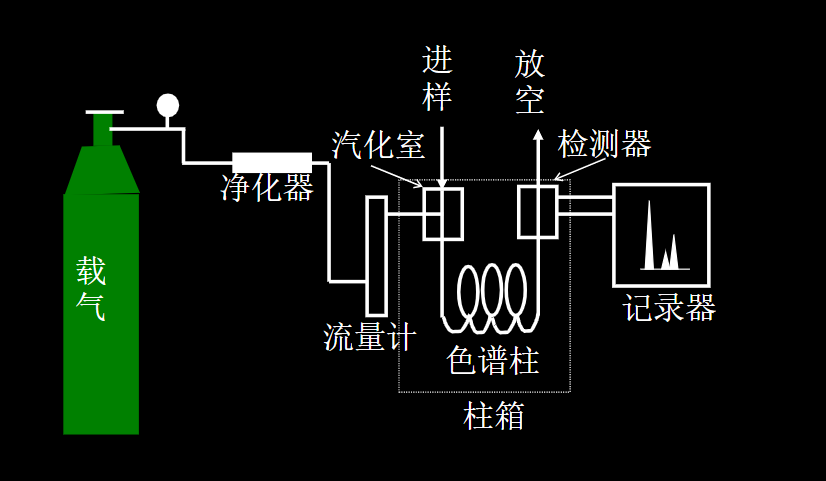
\includegraphics[width=0.7\linewidth]{image/chp1_GC_apa}
	\caption{气相色谱仪}
	\label{fig:chp1gcapa}
\end{figure}
\begin{enumerate}
	\item 载气系统:要求纯净(净化器)、稳定(稳压阀或双路气)。
	
	常用$\ce{H2,N2,He}$。
	\item 进样系统:进样装置和汽化室。
	
	进样通常用微量注射器和进样阀将样品引入。液体样品引入后需要瞬间汽化,汽化在汽化室进行。对汽化室有如下要求:体积小、热容大、对样品无催化作用。
	
	对高分子样品,则采用裂解装置(管式炉、热丝、居里点裂解器等)。
	\item 分离系统:色谱柱和固定相。
	
	色谱柱包括填充柱和毛细管柱。毛细管柱较细长。
	
	固定相有固体固定相和液体固定相。固体固定相是固体吸附剂。液体固定相由担体和固定液组成。
	
	\begin{definition*}{担体}{}
		担体是一种多孔的、化学惰性的固体颗粒,可以提供较大表面积的惰性表面以承担固定液。
	\end{definition*}
	\item 控温系统:控制恒温或程序升温。
	
	$K$是热力学常数,温度越高,$K$值越小,保留时间越短。因此可通过柱温调节分离程度。
	\item 检测器:将分离后各组分的量转变为电信号并记录。
	
	要求灵敏度高、线性范围宽、响应速度快、结构简单、通用性强。
\end{enumerate}

\subsection{气相色谱常用的检测器}
检测器的性能指标:
\begin{itemize}
	\item 灵敏度$S$。样品量变化引起信号变化程度越大,灵敏度越高。$S=\dfrac{\Delta R}{\Delta  Q}$,$R$:峰高或面积;$Q$:浓度或质量
	\item 检测限。三倍噪音相当的物质的量称为检测限。$D=\dfrac{3N}{S}$,$N$为噪音,单位为$\mathrm{mV}$
	\item 线性范围:指检测器信号与样品浓度之间成正比关系的范围。
\end{itemize}

常用检测器:
\begin{enumerate}
	\item 热导检测器(TCD)
	\begin{itemize}
		\item 原理:基于各物质热导系数的不同
		\item 特点:结构简单;灵敏度不高
		\item 检测物质:对所有物质都有响应(无机物和有机物)
	\end{itemize}
	\item 氢火焰离子化检测器(FID)
	\begin{itemize}
		\item 原理:有机物在火焰中电离形成离子流,根据离子流的出现和大小进行分析。
		\item 特点:
		\begin{itemize}
			\item 灵敏度高($10^{-12}\mathrm{g/s}$),线性范围宽
			\item 不能检测惰性气体、空气、$\ce{H2O,CO,CO2,NO,SO2,H2S}$等。
		\end{itemize}
		\item 检测物质:适于有机物的检测
	\end{itemize}
	\item 电子俘获检测器(ECD)
	\begin{itemize}
		\item 原理:载气在$\beta$-射线源下电离形成稳定的基流,卤素、S、P、O等电负性原子捕获电子形成负离子并与载气正离子结合,使基流信号下降,据此检测组分。
		\item 特点:
		\begin{itemize}
			\item 对卤素、S、P、O有很强的响应
			\item 灵敏度高,可用于痕量农药残留的分析
			\item 线性范围较窄
		\end{itemize}
		\item 检测物质:含卤素、S、P、O等电负性较强原子的物质
	\end{itemize}
	\item 火焰光度检测器(FPD)
	\begin{itemize}
		\item 原理:S、P在燃烧中被激发,从而发生特征的光信号(S-394nm,P-526nm)	
		\item 检测物质:含硫、磷的化合物
	\end{itemize}
\end{enumerate}

\subsection{气象色谱的分离}
极性原则(选择固定液):
\begin{itemize}
	\item 非极性组分分离:用非极性固定液,出峰顺序由蒸汽压决定,沸点高的保留时间长。
	\item 中等极性组分分离:用中等极性固定相,沸点与分子间力同时起作用。
	\item 强极性组分分离:用强极性固定相,分子间力起作用,按极性大小出峰,极性小的新出峰。
	\item 极性和非极性分离:用极性固定相,非极性先出峰。
	\item 能形成氢键的试样:选择极性或氢键型固定液,不易形成氢键的后出峰。
\end{itemize}

如何判断极性:

选取两种分析对象A,B:$\beta,\beta’$-氧二丙氰、角沙烷,以待测固定液为固定液制成色谱柱,求三种固定液中的:
\begin{equation*}
	q=\lg⁡\dfrac{t_R (A)}{t_R (B)}
\end{equation*}
则该固定液的相对极性$P_x$为
\begin{equation*}
	P_x=100-100 \dfrac{(q_{\beta\beta}-q_x)}{(q_{\beta\beta}-q_j)}
\end{equation*}

\begin{example}
	已知在柱温为50\textcelsius 和其他给定条件下,测定$t_M=0.42$min。用环己烷与苯在$\beta,\beta’$-氧二丙氰柱上测得$q_1=1.0086$,在角鲨烷上测得$q_2=0.179$,在癸二酸壬酯柱上测的$t_R(\text{环己烷})=4.22$min,$t_R(\text{苯})=6.22$min,计算癸二酸壬酯的相对极性。
\end{example}

\section{高效液相色谱法}
%3.了解高效液相色谱法的特点,熟悉高效液相色谱仪的主要部件及分析流程,理解液相色谱流动相的选择?

气相色谱只适合分析较易挥发、且化学性质稳定的有机化合物,而高效液相色谱法(High Performance Liquid Chromatography, HPLC)则适合于分析那些用气相色谱难以分析的物质,如挥发性差、极性强、具有生物活性、热稳定性差的物质。

特点:
\begin{itemize}
	\item 色谱柱可反复使用,流动相可选择范围宽,流出组分容易收集;
	\item 分离效率高,灵敏度高;
	\item 操作自动化,应用范围广。
\end{itemize}

\subsection{主要部件}
\begin{enumerate}
	\item 输液系统
	\begin{itemize}
		\item 高压输液泵:以稳定的流速或压力将流动相输送到色谱系统。
		\item 在线脱气装置:也使用超声、真空等脱气方式。脱气的目的是去除气泡,保证流动相流速稳定,减小噪音。
		\item 梯度洗脱装置:通过两个输液泵流速的变化,改变流动相洗脱能力,作用与气象色谱的程序升温类似。
	\end{itemize}
	\item 进样系统
	
	通常采用六通阀。
	\item 色谱柱
	
	是核心部件。要求柱效高、柱容量大、性能稳定。柱性能与柱结构、填料特性、填充质量和使用条件有关。
	\item 检测器
	
	连续监测流出物的组成和含量变化的装置。
	\begin{itemize}
		\item 紫外-可见检测器
		\item 荧光检测器:灵敏度高,选择性好,适用于药物、生化样品的分析。
		\item 蒸发光散射检测器:适用于无紫外吸收、无电活性、不发荧光的样品的检测。
		\item 电化学检测器
	\end{itemize}

\end{enumerate}

\subsection{分析流程}
由泵将储液瓶中的溶剂吸入色谱系统,然后输出,经流量与压力测量之后,导入进样器。被测物由进样器注入,并随流动相通过色谱柱,在柱上进行分离后进入检测器,检测信号由数据处理设备采集与处理,并记录色谱图。废液流入废液瓶。遇到复杂的混合物分离(极性范围比较宽)还可用梯度控制器作梯度洗脱。这和气相色谱的程序升温类似,不同的是气相色谱改变温度,而HPLC改变的是流动相极性,使样品各组分在最佳条件下得以分离。

\subsection{流动相的选择}
\begin{itemize}
	\item 对样品有一定溶解度;
	\item 适用于选用的检测器,如用紫外检测时,不能选择对紫外光有吸收的溶剂;
	\item 化学惰性好,液液色谱中不能与固定相互溶,硅胶吸附剂不能用碱性溶剂,氧化铝吸附剂不能用酸性溶剂。
	\item 黏度低。黏度太大会降低样品的扩散系数,导致传质减慢,柱效降低,同时柱压也会升高。
	\item 高纯度。宜采用色谱纯试剂,否则会导致噪音增加,干扰定性、定量。
	\item 安全低毒,环境友好。
\end{itemize}

\section{几种色谱法}
%4.熟悉吸附色谱法、分配色谱法、离子交换色谱法和体积排除色谱法的应用特点,选择分离类型的原则,了解色谱技术在生物分析中的应用。
\subsection{吸附色谱法(absorption chromatography)}

\begin{itemize}
	\item 原理:各组分在固定相表面的吸附作用不同;
	\item 固定相:活性硅胶、氧化铝、活性炭、聚乙烯、聚酰胺等固体吸附剂,所以吸附色谱也称液固吸附色谱。活性硅胶最常用;
	\item 流动相:弱极性有机溶剂或非极性溶剂与极性溶剂的混合物,如正构烷烃(己烷、戊烷、庚烷等)、二氯甲烷/甲醇、乙酸乙酯/乙腈等;
	\item 应用特点:用于结构异构体分离和族分离。如农药异构体分离、石油中烷、烯、芳烃的分离。缺点是易产生不对称峰和拖尾现象。
\end{itemize}

\subsection{分配色谱法}

\begin{itemize}
	\item 原理:样品分子在流动相、固定相间溶解度不同(分配作用)。可分为液-液分配色谱和键合固定相分配色谱。
	\item 固定相:
	\begin{itemize}
		\item 非极性键合固定相:键合在载体表面的功能分子是烷基、苯基等非极性有机分子。如最常用的ODS(十八烷基键合硅胶)柱或$\ce{C18}$柱就是最典型的代表,其极性很小。
		\item 极性键合固定相:键合在载体表面的功能分子是具有二醇基、醚基、氰基、氨基等极性基团的有机分子
	\end{itemize}
	\item 流动相:
	\begin{itemize}
		\item 正相HPLC(normal  phase, HPLC):是由极性固定相和非极性(或弱极性)流动相所组成的HPLC体系。其代表性的固定相是改性硅胶、氰基柱等,代表性的流动相是正己烷。吸附色谱也属正相HPLC。
		\item 反相HPLC(reversed phase, HPLC):由非极性固定相和极性流动相所组成的液相色谱体系,与正相HPLC体系正好相反。其代表性的固定相是十八烷基键合硅胶(ODS柱),代表性的流动相是甲醇和乙腈。
	\end{itemize}
	\item 应用特点:考虑流动相极性、选择性(按接受质子能力、给出质子能力和偶极作用能力分)。
\end{itemize}

\subsection{离子交换色谱法(ion exchange chromatography, IEC)}
\begin{itemize}
	\item 原理: 通过不同离子与交换基团的作用力大小不同(则保留时间不同)来进行分离。
	\item 固定相:离子交换剂,表面有离子交换基团。
	\begin{itemize}
		\item 带负电:分离阳离子。如磺酸基、羧基;
		\item 带正电:分离阴离子。如季铵盐。
	\end{itemize}
	\item 应用特点:适于分离带电的物质,流动相常用含盐的缓冲液,有时也加入有机溶剂以增加某些组分的溶解度。
\end{itemize}



\subsection{体积排除色谱法}

\section{}
%5.了解细管电动色谱、毛细管电泳。





